
\chapter{Introduction}


\section{Overview}

PyLith is is portable, scalable software for simulation of crustal
deformation across spatial scales ranging from meters to hundreds of
kilometers and temporal scales ranging from milliseconds to thousands
of years. Its primary applications are quasi-static and dynamic
modeling of earthquake faulting.

\section{New in PyLith Version \pylithVersionNumber}
\begin{itemize}
\item Added new examples
  \begin{itemize}
  \item \filename{examples/3d/subduction}: New suite of examples for a 3-D
    subduction zone. This intermediate level suite of examples
    illustrates a wide range of PyLith features for quasi-static simulations.
  \item \filename{examples/2d/subduction}: Added quasi-static
    spontaneous rupture earthquake cycle examples (Steps 5 and 6) for
    slip-weakening and rate- and state-friction.
  \item These new examples make use of ParaView Python scripts to
    facilitate using ParaView with PyLith.
  \end{itemize}
\item Improved the PyLith manual
  \begin{itemize}
  \item Added diagram to guide users on which installation method best
    meets their needs.
  \item Added instructions for how to use the Windows Subsystem for
    Linux to install the PyLith Linux binary on systems running
    Windows 10.
  \end{itemize}
\item Fixed bug in generating Xdmf files for 2-D vector
  output. Converted Xdmf generator from C++ to Python for more robust
  generation of Xdmf files from Python scripts.
\item Updated spatialdata to v1.9.10. Improved error messages when
  reading SimpleDB and SimpleGridDB files.
\item Updated PyLith parameter viewer to v1.1.0. Application and
  documentation are now available online
  (\url{https://geodynamics.github.io/pylith_parameters/}). Small fix
  to insure hierarchy path listed matches the one for PyLith.
\item Updated PETSc to v3.7.6. See the PETSc documentation for a
  summary of all of the changes.
\item Switched to using CentOS 6.9 for Linux binary builds to insure
  compatibility with glibc 2.12 and later.
\end{itemize}
The \filename{CHANGES} file in the top-level source directory contains
a summary of features and bugfixes for each release.


\section{History}

PyLith 1.0 was the first version to allow the solution of both
implicit (quasi-static) and explicit (dynamic) problems and was a
complete rewrite of the original PyLith (version 0.8). PyLith 1.0
combines the functionality of EqSim
\cite{Aagaard:etal:2001a,Aagaard:etal:2001b} and PyLith 0.8. PyLith
0.8 was a direct descendant of LithoMop and was the first version that
ran in parallel, as well as providing several other improvements over
LithoMop. LithoMop was the product of major reengineering of Tecton, a
finite-element code for simulating static and quasi-static crustal
deformation. The major new features present in LithoMop included
dynamic memory allocation and the use of the Pyre simulation framework
and PETSc solvers. EqSim was written by Brad Aagaard to solve problems
in earthquake dynamics, including rupture propagation and seismic wave
propagation.

The release of PyLith 1.0 has been followed by additional releases
that expand the number of features as well as improve performance.
The PyLith 1.x series of releases allows the solution of both
quasi-static and dynamic problems in one, two, or three
dimensions. The code runs in either serial or parallel, and the design
allows for relatively easy scripting using the Python programming
language. Material properties and values for boundary and fault
conditions are specified using spatial databases, which permit easy
prescription of complex spatial variations of properties and
parameters. Simulation parameters are generally specified through the
use of simple ASCII files or the command line.  At present, mesh
information may be provided using a simple ASCII file (PyLith mesh
ASCII format) or imported from CUBIT or LaGriT, two widely-used
meshing packages. The elements currently available include a linear
bar in 1D, linear triangles and quadrilaterals in 2D, and linear
tetrahedra and hexahedra in 3D. Materials presently available include
isotropic elastic, linear Maxwell viscoelastic, generalized Maxwell
viscoelastic, power-law viscoelastic, and Drucker-Prager
elastoplastic. Boundary conditions include Dirichlet (prescribed
displacements and velocities), Neumann (traction), point forces, and
absorbing boundaries.  Cohesive elements are used to implement slip
across interior surfaces (faults) with both kinematically-specified
fault slip and slip governed by fault constitutive models. PyLith also
includes an interface for computing static Green's functions for fault
slip.

PyLith 2.0 replaces the finite-element data structures provided by the
C++ Sieve implementation with those provided by the C DMPlex
implementation.  The newly developed DMPlex implementation by the
PETSc developers conforms to the PETSc data manager (DM) interface,
thereby providing tighter integration with other PETSc data
structures, such as vectors and matrices. Other improvements include
significantly reduced memory use and memory balancing.

PyLith is under active development and we expect a number of additions
and improvements in the near future. Likely enhancements will include
additional bulk and fault constitutive models, coupled quasi-static
and dynamic simulations for earthquake cycle modeling, and coupling
between elasticity, heat flow, and/or fluid flow.


\section{PyLith Workflow}

PyLith is one component in the process of investigating problems in
tectonics (Figure \vref{fig:Workflow-summary}). Given a geological
problem of interest, a scientist must first provide a geometrical
representation of the desired structure. Once the structure has been
defined, a computational mesh must be created. PyLith presently
provides three mesh importing options: CUBIT Exodus format, LaGriT GMV
and Pset files, and PyLith mesh ASCII format. The modeling of the
physical processes of interest is performed by a code such as
PyLith. Present output consists of VTK or HDF5/Xdmf files which can be
used by a number of visualization codes (e.g., ParaView, Visit, and
Matlab).

\begin{figure}[htbp]
  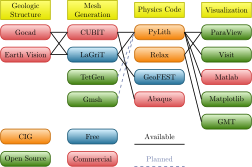
\includegraphics[width=4in]{intro/figs/workflow}
  \caption{Workflow involved in going from geologic structure to
    problem analysis.}
  \label{fig:Workflow-summary}
\end{figure}

\section{PyLith Design}

PyLith is separated into modules to encapsulate behavior and facilitate
use across multiple applications. This allows expert users to replace
functionality of a wide variety of components without recompiling
or polluting the main code. PyLith employs external packages (see
Figure \vref{fig:pylith-dependencies}) to reduce development time
and enhance computational efficiency; for example, PyLith 0.8 ran
two times faster when the PETSc linear solver was used.

\begin{figure}[htbp]
  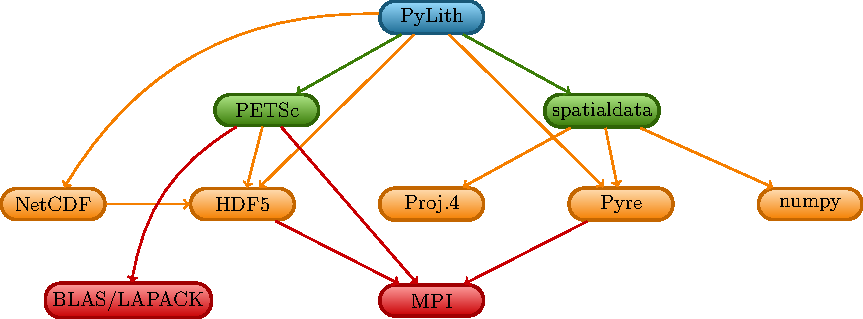
\includegraphics[width=4in]{intro/figs/packages}
  \caption{PyLith dependencies. PyLith makes direct use of several
    other packages, some of which have their own dependencies.}
  \label{fig:pylith-dependencies}
\end{figure}

PyLith is written in two programming languages. High-level code is
written in Python; this rich, expressive interpreted language with
dynamic typing reduces development time and permits flexible addition
of user-contributed modules. This high-level code makes use of Pyre, a
science-neutral simulation framework developed at Caltech, to link the
modules together at runtime and gather user-input. Low-level code is
written in C++, providing fast execution while still allowing an
object-oriented implementation. This low-level code relies on PETSc to
perform operations on matrices and vectors in parallel. We also make
extensive use of two Python packages. SWIG is a package that
simplifies the task of adding C++ extensions to Python code, and FIAT
provides tabulated basis functions and numerical quadrature points.

In writing PyLith 1.0, the code was designed to be object-oriented and
modular. Each type of module is accessed through a specified interface
(set of functions). This permits adding, replacing, and rewriting
modules without affecting other parts of the code. This code structure
simplifies code maintenance and development. Extending the set of code
features is also easier, since developers can create new modules
derived from the existing ones.

The current code design leverages Pyre and PETSc extensively. Pyre
glues together the various modules used to construct a simulation and
specify the parameters. PETSc provides the finite-element data
structures and handles the creation and manipulation of matrices and
vectors. As a result, most of the PyLith source code pertains to
implementing the geodynamics, such as bulk rheology, boundary
conditions, and slip on faults.

PyLith also uses FIAT to tabulate the finite-element basis functions
at the numerical integration (quadrature) points. Nemesis allows
PyLith to run Python using the Message Passing Interface (MPI) for
parallel processing. Additional, indirect dependencies (see Figure
\vref{fig:pylith-dependencies}) include numpy (efficient operations on
numerical arrays in Python), Proj.4 (geographic projections), and SWIG
(calling C++ functions from Python).

During development, tests were constructed for nearly every module
function. These unit tests are distributed with the source code. These
tests are run throughout the development cycle to expose bugs and
isolate their origin. As additional changes are made to the code, the
tests are rerun to help prevent introduction of new bugs. A number of
simple, full-scale tests, such as axial compression and extension,
simple shear, and slip on through-going faults, have been used to test
the code. Additionally, we have run the Southern California Earthquake
Center crustal deformation and several of the spontaneous rupture
benchmarks for strike-slip and reverse-slip to determine the relative
local and global error (see Chapter \vref{sec:benchmarks}).

\subsection{Pyre}

Pyre is an object-oriented environment capable of specifying and launching
numerical simulations on multiple platforms, including Beowulf-class
parallel computers and grid computing systems. Pyre allows the binding
of multiple components such as solid and fluid models used in Earth
science simulations, and different meshers. The Pyre framework enables
the elegant setup, modification and launching of massively parallel
solver applications.

\begin{figure}[htbp]
  \includegraphics[width=4in]{intro/figs/pyre_overview}
  \caption{Pyre Architecture. The integration framework is a set of
    cooperating abstract services.}
  \label{fig:Pyre:Architecture}
\end{figure}

Pyre is a framework, a combination of software and design philosophy
that promotes the reuse of code. In their canonical software design
book, \emph{Design Patterns}, Erich Gamma \textit{et al}. condense
the concept of a framework concept down to, ``When you use a framework,
you reuse the main body and write the code it calls.'' In the context
of frameworks and object-oriented programming, Pyre can be thought
of as a collection of classes and the way their instances interact.
Programming applications based on Pyre will look similar to those
written in any other object-oriented language. The Pyre framework
contains a subset of parts that make up the overall framework. Each
of those parts is designed to solve a specific problem.

The framework approach to computation offers many advantages. It permits
the exchange of codes and promotes the reuse of standardized software
while preserving efficiency. Frameworks are also an efficient way
to handle changes in computer architecture. They present programmers
and scientists with a unified and well-defined task and allow for
shared costs of the housekeeping aspects of software development.
They provide greater institutional continuity to model development
than piecemeal approaches.

The Pyre framework incorporates features aimed at enabling the
scientific non-expert to perform tasks easily without hindering the
expert. Target features for end users allow complete and intuitive
simulation specification, reasonable defaults, consistency checks of
input, good diagnostics, easy access to remote facilities, and status
monitoring. Target features for developers include easy access to user
input, a shorter development cycle, and good debugging support.


\subsection{PETSc}

PyLith 2.x makes use of a set of data structures and routines in PETSc
called \object{DMPlex}, which is still under active
development. \object{DMPlex} provides data structures and routines for
for representing and manipulating computational meshes, and it greatly
simplifies finite-element computations.\object{DMPlex} represents the
topology of the domain. Zero volume elements are inserted along all
fault surfaces to implement kinematic (prescribed) or dynamic
(constitutive model) implementations of fault slip. Material
properties and other parameters are represented as scalar and vector
fields over the mesh using vectors to store the values and sections to
map vertices, edges, faces, and cells to indices in the vector. For
each problem, functions are provided to calculate the residual and its
Jacobian.  All numerical integration is done in these functions, and
parallel assembly is accomplished using the get/set closure paradigm
of the \object{DMPlex} framework. We assemble into PETSc linear
algebra objects and then call PETSc solvers.

PETSc \url{www-unix.mcs.anl.gov/petsc/petsc-as}, the Portable,
Extensible Toolkit for Scientific computation, provides a suite of
routines for parallel, numerical solution of partial differential
equations for linear and nonlinear systems with large, sparse systems
of equations.  PETSc includes solvers that implement a variety of
Newton and Krylov subspace methods. It can also interface with many
external packages, including ESSL, MUMPS, Matlab, ParMETIS, PVODE, and
Hypre, thereby providing additional solvers and interaction with other
software packages.

PETSc includes interfaces for FORTRAN 77/90, C, C++, and Python for
nearly all of the routines, and PETSc can be installed on most Unix
systems. PETSc can be built with user-supplied, highly optimized
linear algebra routines (e.g., ATLAS and commercial versions of
BLAS/LAPACK), thereby improving application performance. Users can use
PETSc parallel matrices, vectors, and other data structures for most
parallel operations, eliminating the need for explicit calls to
Message Passing Interface (MPI) routines. Many settings and options
can be controlled with PETSc-specific command-line arguments,
including selection of preconditions, solvers, and generation of
performance logs.
